\documentclass[11pt,a4paper]{article}

% Compilar com lualatex (UTF-8 nativo). Ex.:
%   lualatex -interaction=nonstopmode relatorio_fase1.tex   (2x)
\usepackage{fontspec}
% Fonte Helvetica (TeX Gyre Heros), igual ao relatorio da AGES (pacote helvet)
\setmainfont{TeX Gyre Heros}
\setsansfont{TeX Gyre Heros}
\usepackage[brazil]{babel}
\usepackage[a4paper,margin=2.5cm]{geometry}
\usepackage{graphicx}
\usepackage[table]{xcolor}
\usepackage{listings}
\usepackage{booktabs}
\usepackage{array}
\usepackage{tikz}
\usetikzlibrary{positioning,arrows.meta,calc,fit}
\usepackage{fancyhdr}
\usepackage[hidelinks]{hyperref}
\usepackage{enumitem}

% ----- Cores e estilo de código -----
\definecolor{corFundo}{RGB}{248,248,248}
\definecolor{corComent}{RGB}{106,115,125}
\definecolor{corKw}{RGB}{167,29,93}
\definecolor{corStr}{RGB}{3,47,98}
\definecolor{corMoldura}{RGB}{210,210,210}
\definecolor{corDestaque}{RGB}{255,245,200}

\lstset{
  basicstyle=\ttfamily\footnotesize,
  backgroundcolor=\color{corFundo},
  frame=single,
  rulecolor=\color{corMoldura},
  breaklines=true,
  breakatwhitespace=false,
  columns=fullflexible,
  keepspaces=true,
  showstringspaces=false,
  extendedchars=true,
  commentstyle=\color{corComent}\itshape,
  keywordstyle=\color{corKw}\bfseries,
  stringstyle=\color{corStr},
  numbers=left,
  numberstyle=\tiny\color{corComent},
  numbersep=8pt,
  tabsize=4,
  captionpos=b,
  xleftmargin=16pt,
}

% Estilo para saídas de terminal / capturas (sem realce de sintaxe)
\lstdefinestyle{saida}{
  language=,
  keywordstyle=\color{black},
  commentstyle=\color{black},
  stringstyle=\color{black},
  numbers=none,
  basicstyle=\ttfamily\scriptsize,
}

\pagestyle{fancy}
\fancyhf{}
\lhead{\small Laboratório de Redes — Fase 1}
\rhead{\small Interceptação de Protocolo}
\cfoot{\thepage}
\renewcommand{\headrulewidth}{0.4pt}

\setlength{\parskip}{0.5em}
\setlength{\parindent}{0pt}

% ---------------------------------------------------------------------------
\begin{document}

% =============================== CAPA ===============================
\begin{titlepage}
\centering
\vspace*{1.5cm}
{\large Pontifícia Universidade Católica do Rio Grande do Sul}\\[0.2cm]
{\large Escola Politécnica}\\[0.2cm]
{\large Laboratório de Redes de Computadores}\\[2.5cm]

\rule{\linewidth}{0.5mm}\\[0.5cm]
{\huge \bfseries Interceptação e Defesa de um\\ Protocolo de Aplicação}\\[0.4cm]
{\Large Fase 1 — Reconhecimento e Escuta Passiva}\\[0.3cm]
{\large Criação da aplicação-alvo e do \textit{sniffer} de tráfego}\\
\rule{\linewidth}{0.5mm}\\[1.5cm]

{\large\bfseries Grupo}\\[0.3cm]
{\large
Gabriel Dienstmann Sieczkowski\\
Lorenzo Hubner Panato\\
Luis Felipe Kvieczinski\\
}
\vfill
{\large Entrega 1 — Demonstração da quebra de confidencialidade}\\[0.3cm]
{\large Outubro de 2026}
\end{titlepage}

\tableofcontents
\newpage

% =============================== 1. OBJETIVO ===============================
\section{Objetivo e escopo}

Este relatório documenta a \textbf{Fase 1} do trabalho, cujo objetivo é
demonstrar, na prática, por que um protocolo de aplicação \textbf{sem proteção}
é vulnerável. Para isso o grupo construiu:

\begin{enumerate}[nosep]
  \item um \textbf{serviço-alvo} próprio — par cliente/servidor que se comunica
        por um protocolo de aplicação \textbf{em texto claro} (autenticação com
        usuário e senha);
  \item um \textbf{interceptador passivo} (\textit{sniffer} de aplicação)
        implementado com \textbf{socket raw}, que lê o tráfego e extrai a
        informação sensível (as credenciais).
\end{enumerate}

A Fase 1 evidencia a \textbf{quebra de confidencialidade}: um observador no mesmo
segmento de rede lê as credenciais sem participar da conexão. O produto não é uma
ferramenta de ataque de uso geral — é uma \textbf{prova de conceito} em
\textbf{ambiente fechado e isolado} (VMs do próprio grupo), cujo propósito
declarado é fundamentar a defesa a ser implementada na Fase 3 (TLS + senhas com
\textit{hash}).

\paragraph{Decisões de projeto.}
\begin{itemize}[nosep]
  \item \textbf{Serviço escolhido:} login/autenticação simples (credenciais em
        texto claro) — carrega informação sensível que a interceptação demonstra
        e que a Fase 3 protegerá.
  \item \textbf{Linguagem:} Python 3, usando \textbf{sockets diretamente}, sem
        frameworks que escondam o socket.
  \item \textbf{Captura:} socket raw \texttt{AF\_PACKET}/\texttt{ETH\_P\_ALL} do
        Linux, com decodificação manual dos cabeçalhos Ethernet, IPv4 e TCP
        (nenhuma biblioteca de captura, como \textit{scapy}, foi utilizada).
\end{itemize}

% =============================== 2. TOPOLOGIA ===============================
\section{Topologia da rede}

O teste é feito em uma \textbf{rede interna/host-only isolada} (sem saída para a
Internet), com três VMs no mesmo domínio de enlace. A \textbf{VM-observador}
opera em \textbf{modo promíscuo}, lendo o tráfego do segmento sem participar da
conexão TCP entre cliente e servidor.

\begin{figure}[h]
\centering
\begin{tikzpicture}[
  vm/.style={draw, rounded corners, align=center, minimum width=3.0cm,
             minimum height=1.4cm, fill=blue!5, thick},
  obs/.style={draw, rounded corners, align=center, minimum width=3.0cm,
              minimum height=1.4cm, fill=red!5, thick},
  font=\small
]
  \node[vm]  (cli) {\textbf{VM-cliente}\\\texttt{cliente.py}\\\texttt{10.0.0.10}};
  \node[vm,right=3.2cm of cli] (srv) {\textbf{VM-servidor}\\\texttt{servidor.py}\\\texttt{10.0.0.20}};
  \node[obs,below=2.2cm of $(cli)!0.5!(srv)$] (obs) {\textbf{VM-observador}\\\texttt{sniffer.py}\\\texttt{10.0.0.30}};

  \draw[-{Latex[length=3mm]}, thick]
     (cli) -- node[above,align=center]{\footnotesize TCP 5050\\\footnotesize \texttt{LOGIN usuario senha}\\\footnotesize (texto claro)} (srv);

  \draw[-{Latex[length=3mm]}, dashed, red!70]
     (obs) -- node[right,align=left,pos=0.55]{\footnotesize escuta\\\footnotesize passiva} ($(cli)!0.5!(srv)$);

  \node[draw, dotted, inner sep=0.55cm, fit=(cli)(srv)(obs)] {};
  \node[align=center, below=0.15cm of obs]
     {\footnotesize\itshape Rede interna isolada (10.0.0.0/24) — sem Internet};
\end{tikzpicture}
\caption{Topologia do laboratório: cliente e servidor conversam em texto claro na
porta TCP 5050; o observador, em modo promíscuo, captura o tráfego do segmento.}
\label{fig:topologia}
\end{figure}

O observador não envia pacotes para a conexão: ele apenas \emph{lê} os quadros que
trafegam no segmento (captura passiva), o que torna o ataque praticamente
indetectável por inspeção de tráfego — ponto retomado na análise da Fase 3.

% =============================== 3. PROTOCOLO ===============================
\section{Protocolo da aplicação}

O protocolo é textual, com \textbf{uma mensagem por linha} terminada por
\texttt{\textbackslash n}. É deliberadamente simples e \textbf{inseguro}: não há
cifragem nem \textit{hash} de senha.

\begin{table}[h]
\centering
\begin{tabular}{@{}llp{6.8cm}@{}}
\toprule
\textbf{Sentido} & \textbf{Mensagem} & \textbf{Significado} \\
\midrule
S $\rightarrow$ C & \texttt{200 AUTH-SERVICE v1 pronto} & banner, ao conectar \\
C $\rightarrow$ S & \texttt{LOGIN <usuario> <senha>} & tentativa de autenticação \\
S $\rightarrow$ C & \texttt{200 OK bem-vindo <usuario>} & credenciais válidas \\
S $\rightarrow$ C & \texttt{401 ERRO credenciais invalidas} & credenciais inválidas \\
S $\rightarrow$ C & \texttt{400 ERRO comando malformado} & sintaxe inválida \\
C $\rightarrow$ S & \texttt{QUIT} & encerra a sessão \\
S $\rightarrow$ C & \texttt{221 tchau} & confirmação de encerramento \\
\bottomrule
\end{tabular}
\caption{Mensagens do protocolo do serviço-alvo.}
\label{tab:protocolo}
\end{table}

A credencial viaja no corpo de um segmento TCP \textbf{sem qualquer proteção}: é
exatamente esse payload que o interceptador reconstrói.

% =============================== 4. IMPLEMENTAÇÃO ===============================
\section{Implementação}

Três programas, todos sobre a biblioteca padrão de \texttt{socket}. O código
completo está no Apêndice~\ref{ap:codigo}.

\subsection{Serviço-alvo: servidor e cliente}

O \textbf{servidor} (\texttt{servidor.py}) abre um socket TCP
(\texttt{AF\_INET}/\texttt{SOCK\_STREAM}), faz \texttt{bind}/\texttt{listen} e
trata cada cliente em uma \textit{thread} dedicada — modelo de concorrência que
já prepara a base para a Fase 2. Como o TCP é um fluxo de bytes sem fronteiras de
mensagem, o servidor mantém um \textit{buffer} e processa o fluxo linha a linha:

\begin{lstlisting}[language=Python,caption={Núcleo do tratamento de LOGIN no servidor (trecho).}]
while b"\n" in buffer:
    linha_bytes, buffer = buffer.split(b"\n", 1)
    linha = linha_bytes.decode(ENCODING, errors="replace").strip()
    partes = linha.split()
    comando = partes[0].upper()
    if comando == "LOGIN":
        usuario, senha = partes[1], partes[2]
        if usuarios.get(usuario) == senha:         # comparação em texto claro
            enviar_linha(conexao, f"200 OK bem-vindo {usuario}")
        else:
            enviar_linha(conexao, "401 ERRO credenciais invalidas")
\end{lstlisting}

O \textbf{cliente} (\texttt{cliente.py}) conecta ao servidor, lê o banner e envia
\texttt{LOGIN <usuario> <senha>}. A linha vai pela rede \textbf{sem cifragem} — é
o dado que o \textit{sniffer} captura.

\subsection{Interceptador passivo (socket raw)}

O \textit{sniffer} (\texttt{sniffer.py}) é o entregável central. Ele abre um
\textbf{socket raw} de camada de enlace e decodifica \textbf{manualmente} cada
quadro:

\begin{lstlisting}[language=Python,caption={Abertura do socket raw e laço de captura (trecho).}]
sock = socket.socket(socket.AF_PACKET, socket.SOCK_RAW, socket.ntohs(ETH_P_ALL))
sock.bind((args.interface, 0))
...
while True:
    quadro = sock.recv(65535)
    ethertype, off = parse_ethernet(quadro)      # Ethernet (14 B)
    if ethertype != ETH_P_IP: continue
    protocolo, ip_org, ip_dst, off = parse_ipv4(quadro, off)   # IPv4 (IHL var.)
    if protocolo != PROTO_TCP: continue
    porta_org, porta_dst, flags, off = parse_tcp(quadro, off)  # TCP (data offset)
    if args.porta not in (porta_org, porta_dst): continue
    payload = quadro[off:]                         # dados da aplicação
\end{lstlisting}

Para cada segmento com payload, o programa imprime um \textbf{número sequencial
de pacote}, origem/destino, \textit{flags} TCP e o conteúdo decodificado; ao
reconhecer uma linha \texttt{LOGIN}, extrai e \textbf{destaca usuário e senha}. A
opção \texttt{-{}-pcap} grava um arquivo \texttt{.pcap} (formato \textit{libpcap}
clássico) que pode ser aberto no Wireshark, com numeração de \textit{frames}
coincidente.

% =============================== 5. DEMONSTRAÇÃO ===============================
\section{Demonstração da quebra de confidencialidade}
\label{sec:demo}

\paragraph{Procedimento.} A demonstração foi conduzida com três hosts isolados
num mesmo segmento — cliente \texttt{10.0.0.10}, servidor \texttt{10.0.0.20} e
observador \texttt{10.0.0.30} — reproduzindo a topologia da
Figura~\ref{fig:topologia}. Para reprodutibilidade, o script
\texttt{demo\_topologia.sh} monta esse segmento com \textit{network namespaces}
do Linux (um switch virtual em modo \textit{hub}) e executa tudo
automaticamente. Com o \textit{sniffer} em escuta na interface do observador
(\texttt{sudo python3 sniffer.py -{}-interface v-obs-lab -{}-porta 5050
-{}-pcap wireshark_capture.pcap}), subiu-se o servidor e executaram-se seis sessões de
cliente: \texttt{alice} (válida), \texttt{bob} (senha errada), \texttt{admin} e
\texttt{carol} (válidas) e, por fim, \texttt{alice}+\texttt{carol} em
\textbf{paralelo}, exercitando a concorrência do servidor.

\paragraph{Resultado.} O interceptador leu, sem participar das conexões, todas as
credenciais em texto claro. Trecho real da saída (sessão de \texttt{alice}):

\begin{lstlisting}[style=saida,caption={Saída real do \textit{sniffer}: credenciais capturadas em texto claro.}]
[pacote #2] 18:14:24  10.0.0.10:51184 -> 10.0.0.20:5050  flags=PSH,ACK  len=25
    payload: 'LOGIN alice S3nh4Secreta'
    !!!!!!!!!!!!!!!!!!!!!!!!!!!!!!!!!!!!!!!!!!!!!!!!!!!!!!!!
    !!! CREDENCIAIS CAPTURADAS EM TEXTO CLARO
    !!!   usuario = alice
    !!!   senha   = S3nh4Secreta
    !!!!!!!!!!!!!!!!!!!!!!!!!!!!!!!!!!!!!!!!!!!!!!!!!!!!!!!!
\end{lstlisting}

O log do servidor confirma a mesma sessão do outro lado:

\begin{lstlisting}[style=saida]
[2026-10-05 18:14:24] + conexao de 10.0.0.10:51184
[2026-10-05 18:14:24]   10.0.0.10:51184 LOGIN OK usuario='alice'
\end{lstlisting}

A saída completa do \textit{sniffer} (todas as seis sessões) está no
Apêndice~\ref{ap:sniffer}.

% =============================== 6. EVIDÊNCIA WIRESHARK ===============================
\section{Evidência de captura com Wireshark (números de pacote)}
\label{sec:wireshark}

O arquivo \texttt{wireshark_capture.pcap} gerado pelo \textit{sniffer} foi aberto com o
Wireshark/\texttt{tshark}. A Tabela~\ref{tab:frames} lista os \textbf{20 primeiros
pacotes com dados} de aplicação (as quatro sessões sequenciais); as linhas
destacadas são os \textbf{frames que carregam credenciais} — visíveis em texto
claro. Nesta captura, cliente = \texttt{10.0.0.10} e servidor =
\texttt{10.0.0.20:5050} (sentido \texttt{C$\rightarrow$S} / \texttt{S$\rightarrow$C}).

\begin{table}[h]
\centering\small
\begin{tabular}{@{}r c r p{7.2cm}@{}}
\toprule
\textbf{Frame} & \textbf{Sentido} & \textbf{Len} & \textbf{Payload (texto claro)} \\
\midrule
1 & S$\rightarrow$C & 27 & \texttt{200 AUTH-SERVICE v1 pronto} \\
\rowcolor{corDestaque} 2 & C$\rightarrow$S & 25 & \texttt{LOGIN alice S3nh4Secreta} \\
3 & S$\rightarrow$C & 23 & \texttt{200 OK bem-vindo alice} \\
4 & C$\rightarrow$S & 5 & \texttt{QUIT} \\
5 & S$\rightarrow$C & 10 & \texttt{221 tchau} \\
6 & S$\rightarrow$C & 27 & \texttt{200 AUTH-SERVICE v1 pronto} \\
\rowcolor{corDestaque} 7 & C$\rightarrow$S & 22 & \texttt{LOGIN bob senhaERRADA} \\
8 & S$\rightarrow$C & 31 & \texttt{401 ERRO credenciais invalidas} \\
9 & C$\rightarrow$S & 5 & \texttt{QUIT} \\
10 & S$\rightarrow$C & 10 & \texttt{221 tchau} \\
11 & S$\rightarrow$C & 27 & \texttt{200 AUTH-SERVICE v1 pronto} \\
\rowcolor{corDestaque} 12 & C$\rightarrow$S & 18 & \texttt{LOGIN admin admin} \\
13 & S$\rightarrow$C & 23 & \texttt{200 OK bem-vindo admin} \\
14 & C$\rightarrow$S & 5 & \texttt{QUIT} \\
15 & S$\rightarrow$C & 10 & \texttt{221 tchau} \\
16 & S$\rightarrow$C & 27 & \texttt{200 AUTH-SERVICE v1 pronto} \\
\rowcolor{corDestaque} 17 & C$\rightarrow$S & 23 & \texttt{LOGIN carol qwerty2026} \\
18 & S$\rightarrow$C & 23 & \texttt{200 OK bem-vindo carol} \\
19 & C$\rightarrow$S & 5 & \texttt{QUIT} \\
20 & S$\rightarrow$C & 10 & \texttt{221 tchau} \\
\bottomrule
\end{tabular}
\caption{Lista de pacotes de \texttt{wireshark_capture.pcap} (4 sessões sequenciais). As
quatro linhas destacadas (\textbf{frames 2, 7, 12 e 17}) contêm as credenciais em
texto claro. Os \textbf{frames 21--30} correspondem às duas sessões simultâneas
(concorrência), com novos \texttt{LOGIN} nos frames 22 e 27.}
\label{tab:frames}
\end{table}

\paragraph{Follow TCP Stream.} Reconstruindo o fluxo TCP da primeira sessão
(frame 2) no Wireshark (\textit{Follow $\rightarrow$ TCP Stream}), toda a troca
aparece legível, incluindo a senha:

\begin{lstlisting}[style=saida,caption={\texttt{tshark -q -z follow,tcp,ascii,0} — sessão de \texttt{alice}.}]
Node 0: 10.0.0.20:5050
Node 1: 10.0.0.10:51184
200 AUTH-SERVICE v1 pronto
LOGIN alice S3nh4Secreta
200 OK bem-vindo alice
QUIT
221 tchau
\end{lstlisting}

As Figuras~\ref{fig:wireshark} e~\ref{fig:follow} mostram a mesma evidência na
interface gráfica do Wireshark: a lista de pacotes filtrada pelos \texttt{LOGIN}
(com o painel de bytes revelando a senha) e a reconstrução completa da sessão.

\IfFileExists{results/wireshark_login.png}{%
\begin{figure}[h]
\centering
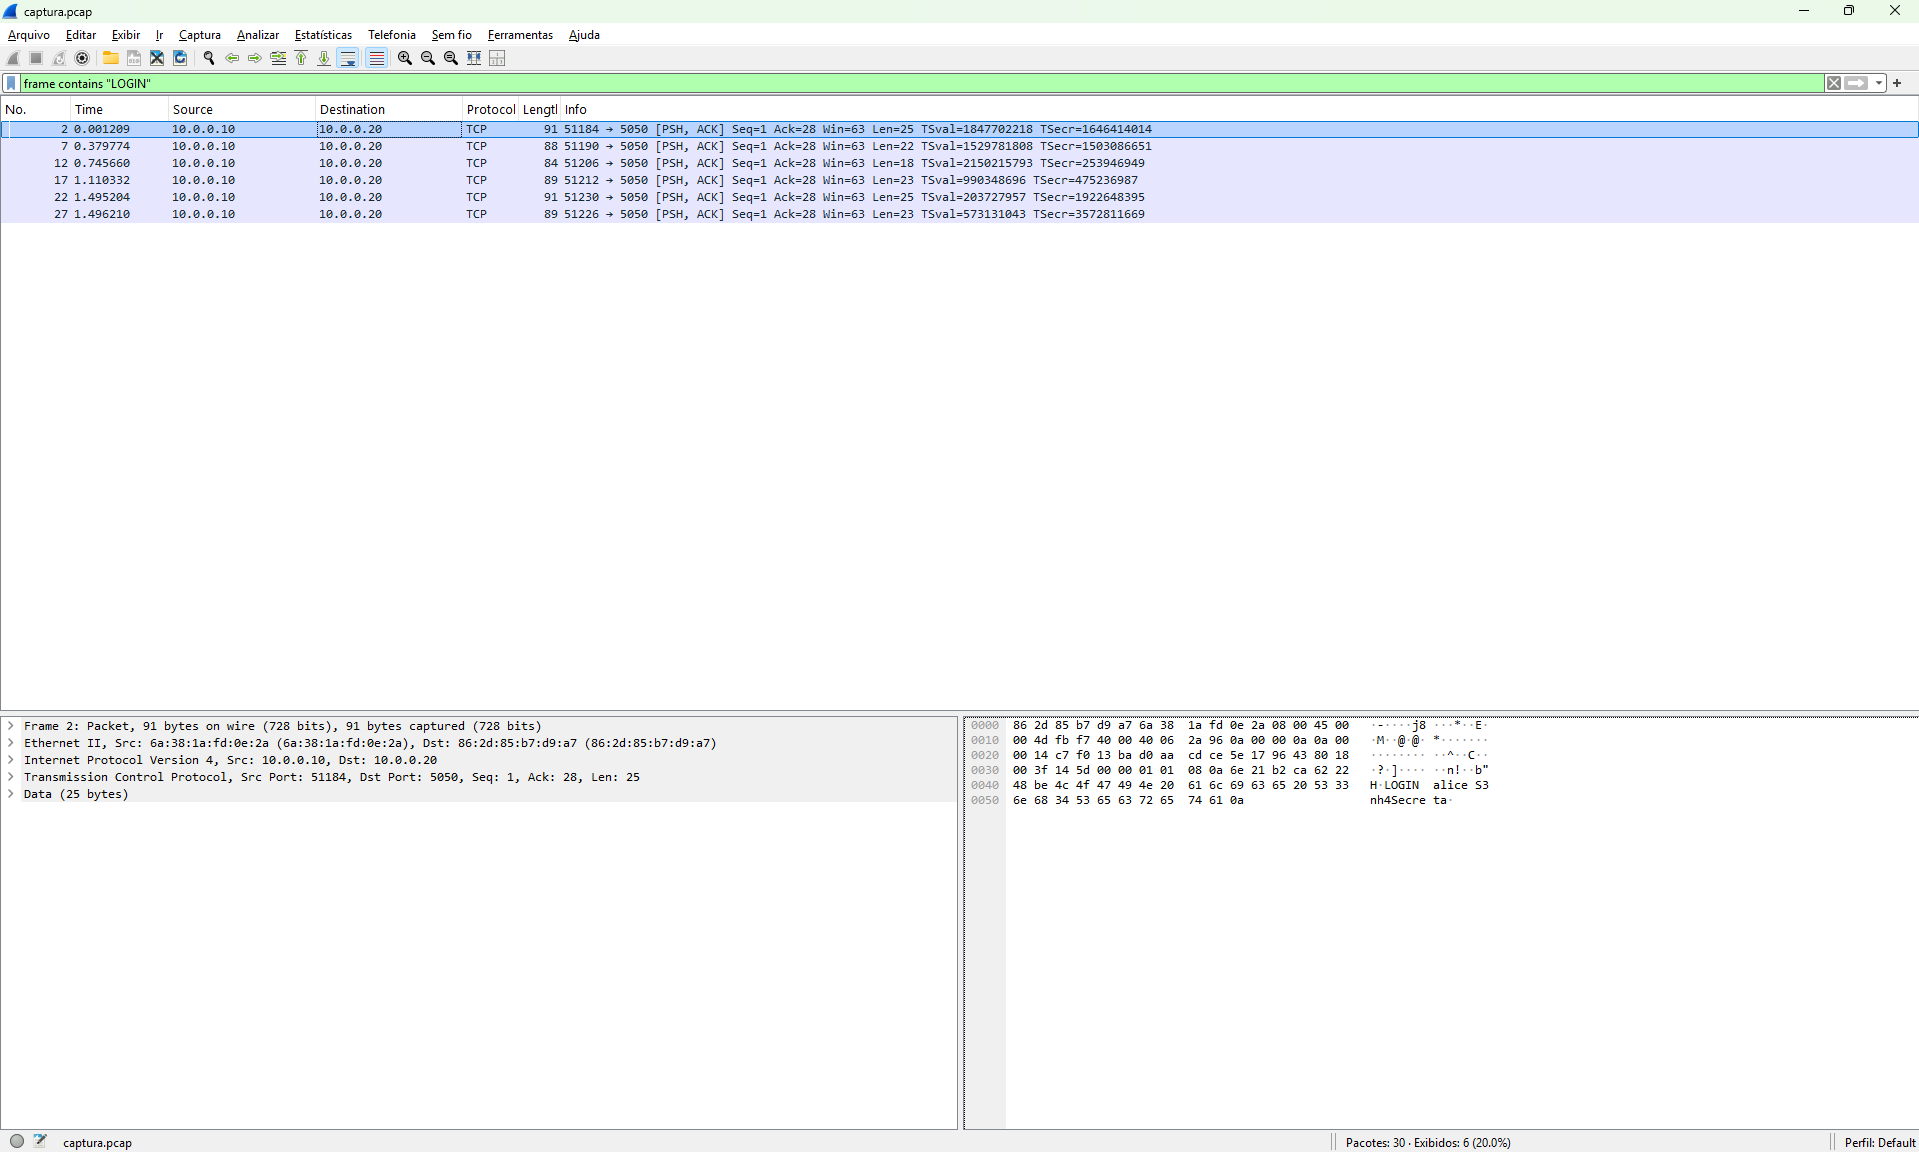
\includegraphics[width=\linewidth,keepaspectratio]{results/wireshark_login.png}
\caption{Wireshark com o filtro \texttt{frame contains "LOGIN"}: os seis pacotes
\texttt{LOGIN} (frames 2, 7, 12, 17, 22 e 27). Com o frame 2 selecionado, o painel
de bytes (canto inferior direito) exibe o conteúdo em texto claro —
\texttt{LOGIN alice S3nh4Secreta}.}
\label{fig:wireshark}
\end{figure}}{}

\IfFileExists{results/wireshark_login_tcp.png}{%
\begin{figure}[h]
\centering
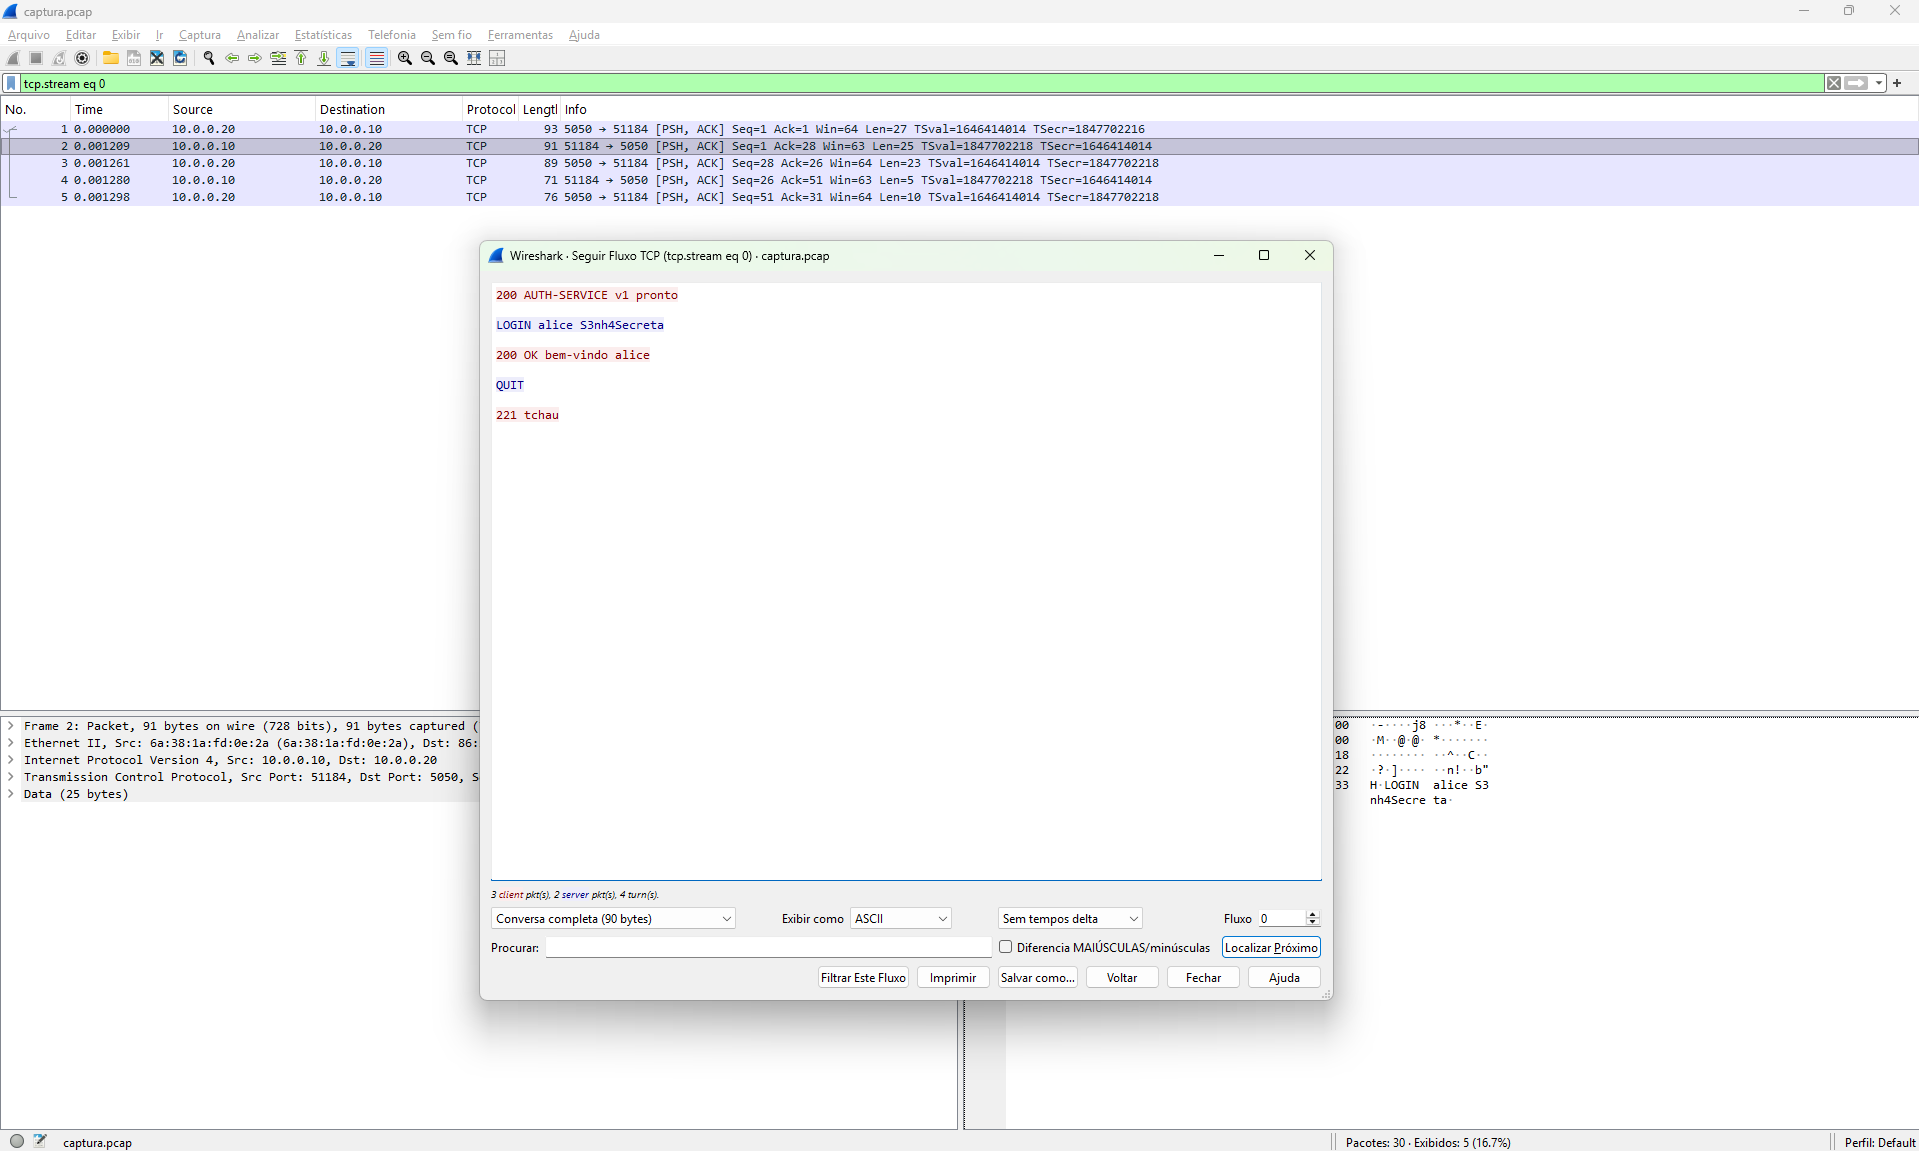
\includegraphics[width=\linewidth,keepaspectratio]{results/wireshark_login_tcp.png}
\caption{Wireshark — \textit{Follow TCP Stream} da sessão de \texttt{alice}: a
conversa inteira é legível (cliente em azul, servidor em vermelho), incluindo a
credencial \texttt{LOGIN alice S3nh4Secreta}. Prova direta da quebra de
confidencialidade.}
\label{fig:follow}
\end{figure}}{}

\paragraph{Sobre o ambiente da captura.} Os três hosts (cliente, servidor e
observador) foram isolados com \textit{network namespaces} do Linux, ligados por
um switch virtual em modo \textit{hub} (sem aprendizado de MAC), de forma que o
observador recebe todo o tráfego do segmento — equivalente a uma VM-observador em
modo promíscuo. Por serem hosts separados numa rede real (e não a interface de
\textit{loopback} \texttt{lo}), a captura não apresenta a duplicação de pacotes
típica do \texttt{lo}: cada segmento aparece \textbf{uma única vez}, como
ocorreria também com três VMs distintas.

% =============================== 7. CONCLUSÃO ===============================
\section{Conclusão}

A Fase 1 cumpre seu objetivo: o par cliente/servidor comunica-se por um protocolo
de aplicação em texto claro, e o interceptador passivo, usando apenas um socket
raw e decodificação manual de Ethernet/IP/TCP, \textbf{reconstrói integralmente o
conteúdo da aplicação e extrai as credenciais} sem participar da conexão. Isso
demonstra, de forma concreta, a \textbf{quebra de confidencialidade} de
protocolos sem proteção.

Como a escuta é \textbf{passiva}, ela não altera o tráfego e é difícil de
detectar apenas observando a rede — motivação direta para as próximas fases: a
Fase 2 mostrará a quebra de \textbf{integridade/autenticação} com um proxy MITM,
e a Fase 3 implementará a defesa (\textbf{TLS} sobre o socket e \textbf{senhas com
hash}), fazendo com que este mesmo \textit{sniffer} deixe de ler o conteúdo.

% =============================== APÊNDICES ===============================
\appendix
\newpage
\section{Instruções de execução (resumo)}
\label{ap:exec}

\begin{lstlisting}[style=saida]
# VM-servidor
python3 servidor.py --host 0.0.0.0 --porta 5050

# VM-observador (Linux, root) -- iniciar ANTES do cliente
sudo python3 sniffer.py --interface eth0 --porta 5050 --pcap wireshark_capture.pcap

# VM-cliente
python3 cliente.py --host 10.0.0.20 --porta 5050 --usuario alice --senha S3nh4Secreta

# Abrir a evidencia no Wireshark
wireshark wireshark_capture.pcap     # ou: tshark -r wireshark_capture.pcap
\end{lstlisting}

Detalhes completos (topologia, modo promíscuo, credenciais de teste) estão no
\texttt{README.md} entregue junto ao código.

\newpage
\section{Código-fonte completo}
\label{ap:codigo}

\subsection{\texttt{servidor.py} — serviço-alvo (servidor)}
\lstinputlisting[language=Python]{../fase1/servidor.py}

\subsection{\texttt{cliente.py} — serviço-alvo (cliente)}
\lstinputlisting[language=Python]{../fase1/cliente.py}

\subsection{\texttt{sniffer.py} — interceptador passivo (socket raw)}
\lstinputlisting[language=Python]{../fase1/sniffer.py}

\subsection{\texttt{demo\_topologia.sh} — topologia de 3 hosts e execução automática}
\lstinputlisting[language=bash]{../fase1/demo_topologia.sh}

\newpage
\section{Saída completa do \textit{sniffer}}
\label{ap:sniffer}
\lstinputlisting[style=saida]{results/sniffer_out_ascii.txt}

\end{document}
